\documentclass{llncs}

\usepackage{fancyhdr}
\usepackage{flushend}
\usepackage{amsfonts,amssymb,amsmath,alltt}
\usepackage{stmaryrd}
\usepackage{xspace}
\usepackage{graphicx}
\usepackage{color}

\usepackage{makeidx}
\pagestyle{plain}
\usepackage[utf8]{inputenc}
\usepackage{url}
\usepackage[english]{babel}


\renewcommand{\ttdefault}{cmtt}
%This version DOES NOT suppress line breaks
% newcommands etc
\newenvironment{ttbox}{\begin{alltt}\ttbraces\small\tt}%
                      {\end{alltt}}
%the new definition of \. suppresses line breaks
\def\ttbraces{\let\.=\nobreak\chardef\{=`\{\chardef\}=`\}\chardef\|=`\\}

\newcommand{\symb}[1]{\makebox{\it #1}} 
\newcommand\ie{i.e.\!\,, }
\newcommand\rel{Re${\cal{L}}$}
\newcommand{\TODO}[1]{\textcolor{red}{\textbf{[TODO:#1]}}}
\newcommand*{\TODOfn}[2][noteC]{\TODO[#1]{[\footnote{\TODO[#1]{#2}}]}}
\newcommand*{\TODOref}[2][todoC]{\TODOfn[#1]{\textbf{BIB-REF}: #2}}
\newcommand\ttand{\mbox{{$\land$}}}
\newcommand\ttor{\mbox{{$\lor$}}}
\newcommand\ttcap{\mbox{{$\cap$}}}
\newcommand\ttcup{\mbox{{$\cup$}}}
\newcommand\ttfun{\mbox{{$\Rightarrow$}}}
\newcommand\ttmimp{\mbox{{$\Longrightarrow$}}}
\newcommand\ttimp{\mbox{{$\longrightarrow$}}}
\newcommand\ttequiv{\mbox{{$\equiv$}}}
\newcommand\ttexists{\mbox{{$\exists$}}}
\newcommand\ttforall{\mbox{{$\forall$}}}
\newcommand\ttneg{\mbox{{$\neg$}}}
\newcommand\ttneq{\mbox{{$\neq$}}}
\newcommand\ttin{\mbox{{$\in$}}}
\newcommand\ttnin{\mbox{{$\notin$}}}
\newcommand\ttImp{\mbox{{$\Longrightarrow$}}}
\newcommand\ttlam{\mbox{\( \lambda \)}}
\newcommand\tttimes{\mbox{\( \times \)}}
\newcommand\ttlbrack{\mbox{\(\llbracket\)}}
\newcommand\ttrbrack{\mbox{\( \rrbracket \)}}
\newcommand\noie{\textit{i.e.},\xspace}
\newcommand\eg{~\textit{e.g.},\xspace}
\newcommand\noeg{\textit{e.g.},\xspace}
\newcommand\ttatI{\mbox{\( @_G \)}}
\newcommand\ttto[1]{\mbox{{$\to^{#1}$}}}
\newcommand\ttleq{\mbox{{$\le$}}}
\newcommand\ttrelI{\mbox{{$\to_{i}$}}}
\newcommand\ttrelIstar{\mbox{{$\to^*$}}}
\newcommand\ttrel[1]{\mbox{{$\to_{#1}$}}}
\newcommand\ttrelstar[1]{\mbox{{$\to_{#1}^*$}}}
\newcommand\ttalpha{\mbox{{$\alpha$}}}
\newcommand\ttsupseteq{\mbox{{$\supseteq$}}}
\newcommand\ttupdownarrow{\mbox{{$\Updownarrow$}}}
\newcommand\tttau{\mbox{{$\tau$}}}
\newcommand\ttsubseteq{\mbox{{$\subseteq$}}}
\newcommand\ttf{\mbox{{$f$}}}
\newcommand\ttvdash{\mbox{{$\vdash$}}}
\newcommand\ttref[1]{\mbox{\(\sqsubseteq_{#1}\)}}
\newcommand\ttNatt{\mbox{{$\mathcal{N}$}}}
\newcommand\ttattand[1]{\mbox{{$\oplus_{\wedge}^{#1}$}}}
\newcommand\ttattor[1]{\mbox{{$\oplus_{\vee}^{#1}$}}}
\newcommand\ttsigma{\mbox{{$\sigma$}}}
\newcommand\ttmref[1]{\mbox{{$\sqsubseteq_{#1}$}}}
\newcommand\ttmeref{\ttmref{\mathcal{E}}}
\newcommand\ttsn{\mbox{{\texttt{s}$_0$}}}
\newcommand\ttsigmap{\mbox{{$\sigma'$}}}
\newcommand\ttecal{\mbox{$\mathcal{E}$}}
\newcommand\ttimg{\mbox{$\triangleleft$}}


\begin{document}
\frontmatter
  
\mainmatter
\title{Modeling and analyzing the Corona-virus warning app with the Isabelle Infrastructure framework}
\author{Florian Kamm\"uller and Bianca Lutz}

\institute{Middlesex University London and\\ Technische Universit\"at Berlin\\
\email{f.kammueller@mdx.ac.uk|bialut@gmail.com}
}
\maketitle
\begin{abstract}
We provide a model in the Isabelle Infrastructure framework of the recently published
Corona-virus warning app. The app supports breaking infection chains by informing users
whether they have been in close contact to an infected person. The app has a decentralized
architecture that supports anonymity of users.
We provide a formal model of the existing app with the Isabelle Infrastructure framework
to show up some natural attacks in a very abstract model. We then use the security
refinement process of the Isabelle Infrastructure framework to highlight how the use of
continuously changing ephemeral ids improves the anonymity.
\end{abstract}

\section{Introduction}
\label{sec:intro}
The German Chancellor Angela Merkel has strongly supported the publication of
the mobile phone Corona warning app by publicly proclaiming that the ``Corona
App deserves your trust'' \cite{bundes:20}. Many millions of mobile phone users
in Germany have downloaded the app with 6 million on the first day.
This app is one amongst many similar application that aim at the very important goal
to ``break infection chains'' by providing timely information of users whether they
have been exposed to close contact with a person that has been infected.

The Corona-virus warning app
%has taken a long time to develop being published only on
%16th June 2020. It
was a quite costly project but this was mainly due to the management of
Telekom and SAP being in the driving seat. But the app has been designed with great
attention on privacy:  a distributed architecture \cite{} has been adopted after a long and
heated debate with supporters of a central architecture. The distributed architecture is
based on a very clever distributed application design whereby users phones are sending
highly anonymized so called ``Ephemeral IDs'' at physical locations via the Bluetooth
protocol. The app saves those IDs of people in close proximity. When at a later date an
infected person reports his infection to a central server, the unique root ID is published
and in the daily check all mobile phones connecting to the central server can download
the root IDs of infected people. Since the Ephemeral IDs can be mapped to the root ID
all Ephemeral IDs that have been saved over the last 14 days allow users phones to
regularly check whether their user has been exposed to an infected person and issue
a warning to the user. The user then needs to contact health autohorities.
%The warning issued by the Corona warning app entitles to
%having a Corona test done (which at the time of writing is not normally possible).

The Isabelle Infrastructure framework \cite{kam:20a} allows modeling and analyzing
architecture and scenarios including physical and logical entities, actors, and policies
within the interactive theorem prover Isabelle supported with temporal logic, Kripke
structures, and attack trees. It has been applied for example to Insider analysis in
airplanes \cite{kam:20b}, privacy in IoT healthcare \cite{kam:18b}, and recently also
to blockchain protocols \cite{kn:20}.

%{Motivation: Why bother re-engineering a formal specification for a nicely developed privacy oriented app? physical aspects (adoption rate), formal proof etc}
The technical advantage of modeling an application in the Isabelle Insider framework lies
in (a) having explicit representations of infrastructures, actors and policies in a
formal model that (b) allows additional automated verification of security properties
within the interactive theorem prover Isabelle.
Although the Corona-virus app has been produced based on a sophisticated security
concept conceived by experts in the field, to our knowledge, no formal verification
has been involved. Even if a ``post-production'' formal specification seems pointless,
it allows to reveal weak points of the architecture, show that the measures that have
been conceived are suitable to cover those weak points. Thereby, we believe
that our current work is useful to increase the trust in the Corona-virus app necessary for
its wide adoption which in turn is crucial for it to be efficient.

The contributions of this paper are (a) formal re-engineering of the Corona-virus warning app
(b) providing an additional security and privacy analysis with interactice theorem proving
certification of a novel view on the system architecture including actors, locations, and policies,
(c) an formal definition of a security refinement process that allows to improve a system
based on attacks found by the attack tree analysis.

In this paper, we first provide some background in Section \ref{sec:background}:
we give a detailed overview of the development history %and security and privacy
ajnd relevant parts of the Corona-virus warning app (Section \ref{sec:history})
We then introduce the Isabelle Infrastructure framework (Section \ref{sec:isainf}).
Next, we present our model (Section \ref{sec:model}) and analysis of privacy and
attacks (Section \ref{sec:ana}). The found attck on the first abstract specification
motivates refinement. The formal definition of refinement for the Isabelle Infrastructure
framework is introduced and illustrated on the Corona-virus warning app (Section \ref{sec:ref})
before drawing some conclusions (Section \ref{sec:concl}).

The formal model in the Isabelle insider framework is fully mechanized and proved in
Isabelle (sources available \cite{kam:18smc}). 

\section{Background and related work}
\label{sec:background}
\subsection{DP-3T and PEPP-PT}
\label{sec:history}
This paper is mainly concerned with the architecture and protocols proposed by the
Decentralized Privacy-Preserving Proximity Tracing project (DP-3T).
The main reason to focus on this particular family of protocols is the
\textit{Exposure Notification Framework}, jointly published by Apple and Google, that adopts
the main core principles of the DP-3T proposal. This API is not only used in the German
Corona-virus warning app but has the potential of being widely adopted in future
app developments that might emerge due to the reach of players like Apple and Google.

There are, however, competing architectures noteworthy, namely protocols developed under the
roof of the \textit{Pan-European Privacy-Preserving Proximity Tracing} project (PEPP-PT), e.g.
PEPP-PT-ROBERT \TODOref{ROBERT github repository} and PEPP-PT-NTK\TODOref{NTK ???; mentioned in
  ``Response to Analysis of DP-3T''}.

Neither DP-3T nor PEPP-PT are synonymous for just one single protocol. Each project endorses
different protocols with unique properties in terms of privacy and data protection.
Yet, on a higher level of abstraction, it seems feasible to distinguish two basic architectures:
protocols as endorsed by PEPP-PT might be characterized as centralized architectures whereas
DP-3T-inspired protocols follow a (more) decentralized approach.\footnote{%
  As we will see, DP-3T involves a central backend server. It is decentralized with regard to
  collection and evaluation of contact information:
  In centralized architectures the server provides a risk scoring services, whereas decentralized
  approaches rely on local risk assessment and, thus, do not need to share contact information with
  the backend.}

\subsubsection{Basic DP-3T protocol: How does it work?}
%  How does it relate to ENF/CWA? (broad strokes)}
%
Upon installation, the app generates secret daily seeds to derive so called \textit{Ephemeral IDs}
(EphIDs) from them. EphIDs are generated locally with cryptographic methods and cannot be connected
to one another but only reconstructed from the secret seed they were derived from.

During normal operation each client broadcasts its EphIDs via Bluetooth whilst scanning for
EphIDs broadcasted by other devices in the vicinity. Collected EphIDs are stored locally along
with associated metadata such as signal attenuation and date. In DP-3T the contact information
gathered is never shared but only evaluated locally (on the device).

If patients are tested positive on the Corona-virus, they are entitled to upload specific data to a
central backend server. This data is accumulated by the backend server and redistributed to all
clients regularly to provide the means for local risk scoring, i.\,e., determining whether collected
EphIDs match those broadcasted by now-confirmed Corona-virus patients during the last, e.\,g., 14, 
days.

In the most simple (and insecure) protocol proposed by DP-3T
\TODOref{Low-cost decentralized proximity tracing; DP-3T Whitepaper p. 14ff}
this basically translates into publishing the daily seeds used to derive EphIDs from.
Aside from additional security measures,
%\TODOfn[styC]{In short: I want to name it but don't talk about it (since we're not really concerned with% this level of detail). But this sounds just sh...}
like signing content the server provides as a general rule, the protocol implemented by ENF and,
hence, CWA follows this low-cost design.\TODOref{CWA solution architecture ($\rightarrow$ github:CWA); probably ENF specification} DP-3T proposes two other, more sophisticated protocols that improve
privacy and data protection properties to different degrees but are more costly.
%TODOfn[styC]{``complicated'' sounds lame but ``costly'' is, perhaps, to simple/literal} to set up.


\subsection{Isabelle Infrastructure framework}
\label{sec:isainf}
%\TODO{Adapt: this is copied from FMBC paper}
The Isabelle Infrastructure is built in the interactive generic theorem prover
Isabelle/HOL \cite{npw:02}. As a framework, it supports formalisation and proof of
systems with actors and policies. It originally emerged from verification of insider 
threat scenarios but it soon became clear that the theoretical concepts, like temporal
logic combined with Kripke structures and a generic notion of state transitions were
very suitable to be combined with attack trees into a formal security engineering process
\cite{suc:16} and framework \cite{kam:19a}.

\subsubsection{Overview}
\label{sec:isainfover}
Figure \ref{fig:theorystruc} gives an overview of the Isabelle Infrastructure 
framework with its layers of object-logics -- each level below embeds the one
above showing the novel contribution of this paper in blue on the top. 
\begin{figure}
\begin{center}
  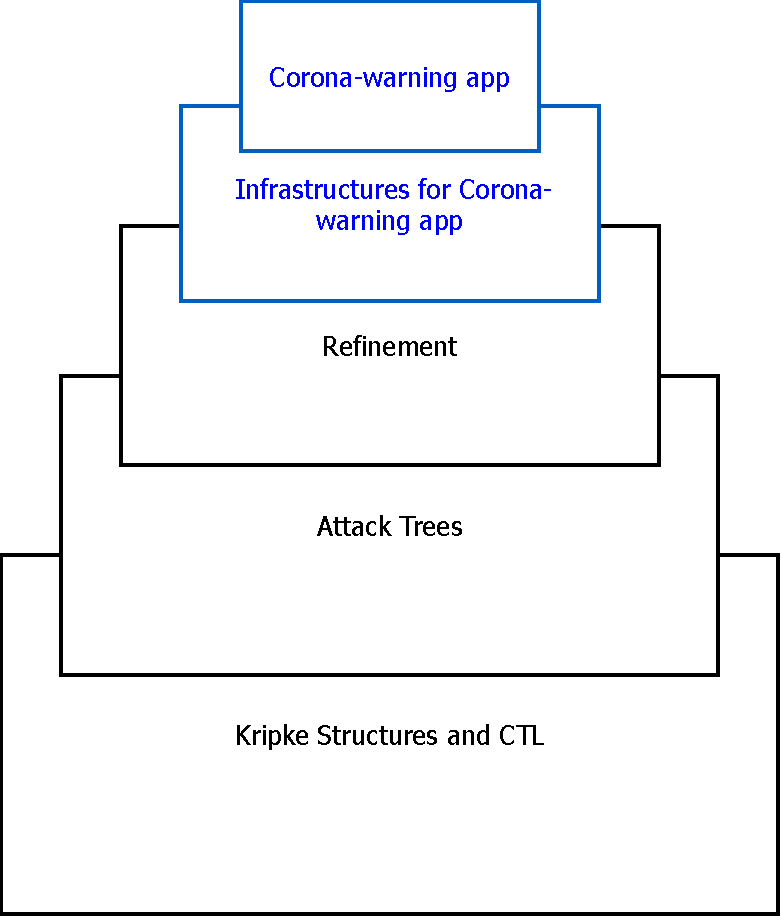
\includegraphics[scale=.5]{theory_structure.pdf}
\end{center}
%\vspace{-.5cm}
\caption{Generic Isabelle Infrastructure framework applied to Corona-warning app.}
\label{fig:theorystruc}
\end{figure}

\subsubsection{Instantiation of Framework}
The formal model of the Corona-warning app uses the Isabelle Infrastructure framework instantiating it
by reusing its concept of {\it actors} for users and smartphones whereby locations correspond
to physical locations. The Ephermeral IDs, their sending and change is added to Infrastructures
by slightly adapting the basic state type of infrastructure graphs and accordingly the semantic rules
for the actions move, get, and put. The details of the newly adapted Infrastructure are
presented in Section \ref{sec:model}.
Technically, an Isabelle theory file \texttt{Infrastructure.thy} builds on top of the theories for Kripke 
structures and CTL (\texttt{MC.thy}), attack trees (\texttt{AT.thy}), and security refinement 
(\texttt{Refinement.thy}). Thus all these concepts can be used to specify the formal model
for the Corona-virus warning app, express relevant and interesting properties, and conduct
interactive proofs (with the full support of the powerful and highly automated proof support
of Isabelle).
%The Corona-virus warning app theory itself is an adaptation of the Infrastructure theory of the 
%Isabelle Infrastructure framework and reuses (or slightly adapts) existing concepts. 
%In the remainder of this paper, we introduce the model that we conceived for . 
All Isabelle sources are available online \cite{kam:20gitsc}.

\subsubsection{Refinement}
An interesting feature that has been integrated into the Isabelle Infrastructure
framework motivated by security engineering formal specifications for IoT healthcare
system is  is an extension of the formal specifciation process introducing
refinement of Kripke structures \cite{kam:19a,kam:20a}. It refines a system model based on a 
formal definition of a combination of trace refinement and structural 
refinement (or datatype refinement). The definition allows to prove property preservation results 
crucial for an iterative development process.
The refinements of the system specification  can be interleaved with attack 
analysis while security properties can be proved in Isabelle. In each iteration
security qualities are accumulated while continuously attack trees scrutinize
the design.


\section{Model}
\label{sec:model}

\section{Analysis}
\label{sec:ana}

\section{Refinement}
\label{sec:ref}
%\TODO{This section is just copied over from arxive paper - adapt}
Intuitively, a refinement changes some aspect of the type of
the state, for example, replaces a data type by a richer datatype or
restricts the behaviour of the actors. The former is expressed directly 
by a mapping of datatypes, the latter is incorporated into the state
transition relation of the Kripke structure that corresponds to the 
transformed model.
%This relationship between the Kripke structure can be better understood
%visually (see Figure \ref{fig:modtrans})
In other words, we can encode a refinement within our framework
as a relation on Kripke structures that is parametrized additionally by
a function that maps the refined type to the abstract type.
The direction ``from refined to abstract'' of this type mapping may seem 
curiously counter-intuitive. However, the actual refinement is given by the 
refinement that uses this function as an input. The refinement
then refines an abstract to a more concrete system specification. 
The additional layer for the refinement 
%(the red box in Figure \ref{fig:theorystruc})
can be formalised in Isabelle as a
%second\footnote{The first refinement 
%relation in this framework is on attack trees summarized in Section \ref{sec:at}.} 
refinement relation 
$\sqsubseteq_{\mathcal{E}}$. 
The relation \texttt{mod\_trans} is typed as a relation over triples --
a function from a threefold Cartesian product to \texttt{bool}, the 
type containing true and false only.  
The type variables $\sigma$ and $\sigma'$ input to the type constructor 
\texttt{Kripke} represent the abstract state type and the concrete state type. 
Consequently, the middle element of the triples selected by the relation 
\texttt{mod\_trans} is a function of type $\sigma' \Rightarrow \sigma$ 
mapping elements of the refined state to the abstract state.
The expression in quotation marks after the type is again the
infix syntax in Isabelle that allows the definition of mathematical notation
instead of writing \texttt{mod\_trans} in prefix manner. This nicer infix
syntax is already used in the actual definition.
Finally, the arrow \texttt{\ttImp} is the implication of Isabelle's  meta-logic
while $\ttimp$ is the one of the {\it object} logic HOL. 
They are logically equivalent but of different
types: within a HOL formula $P$, for example, as below $\forall x. P \ttimp Q$, only the implication $\ttimp$
can be used.
\begin{ttbox}
 mod_trans ::  (\ttsigma Kripke \tttimes (\ttsigma' \ttfun \ttsigma) \tttimes \ttsigma' Kripke) 
               \ttfun bool                  ("_ \ttmref{(\_)} _")
  K \ttmeref K' \ttequiv \ttforall s' \ttin states K'. \ttforall s \ttin init K'. 
             s \ttrelstar{\sigma'} s' \ttimp \ttecal(s) \ttin init K 
             \ttand \ttecal(s) \ttrelstar{\sigma} \ttecal(s')
\end{ttbox}
The definition of \texttt{K \ttmeref\, K'} states that for any state $s$ 
of the refined Kripke structure that can be reached by the state transition
in zero or more steps from an initial state $s_0$ of the refined Kripke 
structure, the mapping ${\mathcal E}$ from the refined to the abstract 
model's state must preserve this reachability, i.e., the image of
$s_0$ must also be an initial state and from there the image of $s$
under ${\mathcal E}$ must be reached with $0$ or $n$ steps.

\subsection{Property Preserving System Refinement}
A first direct consequence of this definition is the following lemma
where the operator \texttt{$\ttimg$} in \texttt{\ttecal\ttimg(init K')}
represents function image, that is the set, $\{\ttecal(x). x \in \texttt{init K'}\} $.
\begin{ttbox}
{\bf{lemma}} init_ref: K \ttmeref K' \ttImp \ttecal\ttimg(init K') \ttsubseteq init K
\end{ttbox}
A more prominent consequence of the definition of refinement 
is that of property preservation. Here, we show that refinement preserves the
CTL property of ${\sf EF} s$ which means that a reachability property true in the
refined  model \texttt{K'} %has also been 
is already true in the abstract model.
A state set $s'$ represents a property %since we use 
in the predicate transformer view of properties as sets of states. 
The additional condition on initial states ensures that we cannot ``forget'' them. 
%initial states.
%The theorem states that, if the 
%property \texttt{{\sf EF} s'} is true in the concrete model its  has been true 
%can be reached from the initial state in 
%\texttt{K'} then it is also possible  to reach the image of this property
% in the abstract Kripke structure \texttt{K}.
\begin{ttbox}
{\bf{theorem}} prop_pres: 
   K \ttmeref K'  \ttImp init K \ttsubseteq \ttecal\ttimg(init K') \ttImp
   \ttforall s' \ttin Pow(states K'). K' \ttvdash {\sf EF} s' 
              \ttimp K \ttvdash {\sf EF} (\ttecal\ttimg(s'))
\end{ttbox}
It is remarkable, that our definition of refinement by Kripke 
structure refinement entails property preservation and makes it possible 
to prove this as a theorem in Isabelle once for all, i.e., as a meta-theorem.
However, this is due to the fact that our generic definition of state transition
allows to explicitly formalise such sophisticated concepts like reachability.
For practical purposes, however, the proof obligation of showing that
a specific refinement is in fact a refinement is rather complex
justly because of the explicit use of the transitive closure of the state
transition relation.
In most cases, the refinement will be simpler. Therefore, we offer
additional help by the following theorem that uses a stronger characterisation
of Kripke structure refinement and shows that our refinement follows
from this.
\begin{ttbox}
{\bf{theorem}} strong_mt: 
\ttecal\ttimg(init K') \ttsubseteq init K \ttand s \ttrel{\sigma'} s' \ttimp \ttecal(s) \ttrel{\sigma} \ttecal(s') 
\ttImp K \ttmeref K'
\end{ttbox}
This simpler characterisation is in fact a stronger one: we could have $s \ttrel{\sigma'} s'$ 
in the refined Kripke structure \texttt{K'} and $\neg(\ttecal(s) \ttrel{\sigma} \ttecal(s'))$
but neither $s$ nor $s'$ are reachable from initial states in \texttt{K'}.
For cases, where we want to have the simpler one-step proviso but still need 
reachability we provide a slightly weaker version of \texttt{strong\_mt}.
\begin{ttbox}
{\bf{theorem}} strong_mt':  
\ttecal\ttimg(init K') \ttsubseteq init K \ttand (\ttexists s0 \ttin init K'. s0  \ttrelIstar s)
 \ttand s \ttrel{\sigma'} s' \ttimp \ttecal(s) \ttrel{\sigma} \ttecal(s') \ttImp K \ttmeref K'
\end{ttbox}

This idea of property preservation coincides with the classical idea of
trace refinement as it is given in process algebras like CSP. In this view,
the properties of a system are given by the set of its traces. Now, a refinement
of the system is given by another system that has a subset of the traces of the 
former one.
Although the principal idea is similar, we greatly extend it since our notion
additionally incorporates refinement. Since we include a state map 
\texttt{\ttsigma'\ttfun \ttsigma} in our refinement map, we additionally
allow structural refinement: the state map generalises the basic idea of
trace refinement by traces corresponding to each other but allows additionally
an exchange of data types. 
As we see in the application to the case study, the refinement steps may
sometimes just specialise the traces: in this case the state map 
\texttt{\ttsigma'\ttfun \ttsigma} is just identity. 

In addition, as we can observe in the following example in the second refinement
step, we also have a simple implicit version of {\it action refinement}. In an
action refinement, traces may be refined by combining consecutive system events
into atomic events thereby reducing traces. This will be detailed on the example
below.

\section{Refining the Specification}
\label{sec:corref}

\section{Conclusions}
\label{sec:concl}
\subsection{Protection goals of attacks}

\subsection{Relevance of the approach}


\bibliographystyle{abbrv}
\bibliography{insider}

\end{document}
